\documentclass[aip,apl,amsmath,amssymb,reprint,longbibliography]{revtex4-1}

\usepackage{graphicx}
\usepackage{bm}
\usepackage[colorlinks=true,allcolors=blue,breaklinks=true]{hyperref}
\usepackage{xurl}

%% generated by rapid/numbers.py -- do not edit
\newcommand{\AdjJacErr}{1.8\times 10^{-8}}
\newcommand{\AdjDotErr}{2.1\times 10^{-16}}
\newcommand{\AdjMapErr}{9.3\times 10^{-10}}
\newcommand{\CondNum}{3.9}
\newcommand{\SigNd}{0.03}
\newcommand{\SigEps}{0.016}
\newcommand{\SigN}{0.059}
\newcommand{\NdRelErr}{7}
\newcommand{\RmseNd}{0.095}
\newcommand{\RmseEps}{0.016}
\newcommand{\RmseN}{0.059}
\newcommand{\MapIter}{4}
\newcommand{\MapIterMax}{15}
\newcommand{\NattooRatio}{6.5}
\newcommand{\NattooRatioSD}{1.1}
\newcommand{\NattooScatter}{16}
\newcommand{\NattooRatioALD}{7.4}
\newcommand{\NattooRatioSputt}{5.6}
\newcommand{\ndALDag}{7.3\times 10^{12}}
\newcommand{\LDALDag}{3.7}
\newcommand{\muceilALDag}{29}
\newcommand{\ndALDan}{5.4\times 10^{12}}
\newcommand{\LDALDan}{4.3}
\newcommand{\muceilALDan}{33}
\newcommand{\ndSPag}{2.2\times 10^{13}}
\newcommand{\LDSPag}{2.1}
\newcommand{\muceilSPag}{14}
\newcommand{\ndSPan}{1.5\times 10^{13}}
\newcommand{\LDSPan}{2.6}
\newcommand{\muceilSPan}{19}
\newcommand{\DeficitLo}{74}
\newcommand{\DeficitHi}{479}
\newcommand{\EdgeN}{2.3\times 10^{12}}
\newcommand{\EdgeNerr}{7.6\times 10^{11}}
\newcommand{\EdgeStrain}{0.000}
\newcommand{\EdgeStrainErr}{0.014}
\newcommand{\EdgeStrainBound}{0.03}
\newcommand{\SpotStrain}{0.134}
\newcommand{\SpotStrainErr}{0.014}
\newcommand{\SpotN}{3.6\times 10^{11}}
\newcommand{\NaiveStrain}{0.10}
\newcommand{\GammaLA}{2.30}
\newcommand{\dwTwoLA}{20.9}
\newcommand{\dwAeps}{5.1}
\newcommand{\LeverRatio}{4.1}
\newcommand{\EdgeNspread}{1}
\newcommand{\OvertoneBound}{16}
\newcommand{\NaiveTwoLA}{2.1}
\newcommand{\GBstrain}{0.39}
\newcommand{\GBstrainRef}{0.6}
\newcommand{\DosOneRef}{56.5}
\newcommand{\DosOnePred}{52}
\newcommand{\DosTwoRef}{8.5}
\newcommand{\DosTwoPred}{27}
\newcommand{\YangWSTwo}{67}
\newcommand{\YangWSeTwo}{42}
\newcommand{\SigmaLine}{2.3\times 10^{6}}
\newcommand{\Wedge}{10}
\newcommand{\Vov}{1.5}
\newcommand{\WcHaloSiOThreeH}{<5}
\newcommand{\WcChgSiOThreeH}{763}
\newcommand{\WcBothSiOThreeH}{765}
\newcommand{\WcHaloSiONinety}{<5}
\newcommand{\WcChgSiONinety}{265}
\newcommand{\WcBothSiONinety}{269}
\newcommand{\WcHaloSiOThirty}{6}
\newcommand{\WcChgSiOThirty}{96}
\newcommand{\WcBothSiOThirty}{100}
\newcommand{\WcHaloHfO}{14}
\newcommand{\WcChgHfO}{7}
\newcommand{\WcBothHfO}{17}
\newcommand{\WcHfOwFive}{15}
\newcommand{\WcHfOwTwenty}{21}
\newcommand{\IonMoSTwentyfive}{326}
\newcommand{\IonMoSFortythree}{398}
\newcommand{\IonMoSSeventyfive}{442}
\newcommand{\IonMoSWide}{497}
\newcommand{\IonWSTwo}{576}
\newcommand{\IonWSeTwo}{384}
\newcommand{\WcRIE}{17}
\newcommand{\WcHIM}{379}
\newcommand{\WcSiOThreeH}{765}
\newcommand{\dVTSiOThreeH}{25.29}
\newcommand{\WcSiONinety}{269}
\newcommand{\dVTSiONinety}{7.58}
\newcommand{\WcSiOThirty}{100}
\newcommand{\dVTSiOThirty}{2.53}
\newcommand{\WcHfO}{17}
\newcommand{\dVTHfO}{0.13}
\newcommand{\WcMoSTwo}{17}
\newcommand{\WcWSTwo}{14}
\newcommand{\WcMoSeTwo}{18}
\newcommand{\WcWSeTwo}{17}
\newcommand{\dVTLiu}{3.16}
\newcommand{\gEMoSTwo}{1.01}
\newcommand{\gAMoSTwo}{0.63}
\newcommand{\CAMoSTwo}{0.59}
\newcommand{\UdefMoSTwo}{0.285}
\newcommand{\CTwoDMoSTwo}{151}
\newcommand{\wEdftMoSTwo}{380}
\newcommand{\wAdftMoSTwo}{405}
\newcommand{\gapMoSTwo}{1.71}
\newcommand{\dgapMoSTwo}{100}
\newcommand{\gLAMoSTwo}{2.30}
\newcommand{\gAdftMoSTwo}{0.63}
\newcommand{\gLApredMoSTwo}{2.30}
\newcommand{\gEWSTwo}{1.05}
\newcommand{\gAWSTwo}{0.65}
\newcommand{\CAWSTwo}{2.92}
\newcommand{\UdefWSTwo}{0.285}
\newcommand{\CTwoDWSTwo}{165}
\newcommand{\wEdftWSTwo}{350}
\newcommand{\wAdftWSTwo}{418}
\newcommand{\gapWSTwo}{1.87}
\newcommand{\dgapWSTwo}{122}
\newcommand{\gLAWSTwo}{2.34}
\newcommand{\gAdftWSTwo}{0.65}
\newcommand{\gLApredWSTwo}{2.34}
\newcommand{\gEMoSeTwo}{1.00}
\newcommand{\gAMoSeTwo}{0.66}
\newcommand{\CAMoSeTwo}{0.31}
\newcommand{\UdefMoSeTwo}{0.285}
\newcommand{\CTwoDMoSeTwo}{124}
\newcommand{\wEdftMoSeTwo}{281}
\newcommand{\wAdftMoSeTwo}{237}
\newcommand{\gapMoSeTwo}{1.48}
\newcommand{\dgapMoSeTwo}{88}
\newcommand{\gLAMoSeTwo}{3.07}
\newcommand{\gAdftMoSeTwo}{0.66}
\newcommand{\gLApredMoSeTwo}{3.07}
\newcommand{\gEWSeTwo}{1.07}
\newcommand{\gAWSeTwo}{0.68}
\newcommand{\CAWSeTwo}{0.95}
\newcommand{\UdefWSeTwo}{0.285}
\newcommand{\CTwoDWSeTwo}{135}
\newcommand{\wEdftWSeTwo}{243}
\newcommand{\wAdftWSeTwo}{245}
\newcommand{\gapWSeTwo}{1.57}
\newcommand{\dgapWSeTwo}{110}
\newcommand{\gLAWSeTwo}{3.15}
\newcommand{\gAdftWSeTwo}{0.68}
\newcommand{\gLApredWSeTwo}{3.15}
\newcommand{\ScPsiErr}{1.8\times 10^{-16}}
\newcommand{\ScElecErr}{1.2\times 10^{-15}}
\newcommand{\ScContErr}{2.7\times 10^{-15}}
\newcommand{\ScSquareErr}{0.2}
\newcommand{\ScCq}{68}
\newcommand{\ScCqCorr}{3.3}
\newcommand{\ScRatio}{0.64}
\newcommand{\ScRatioSpread}{0.05}
\newcommand{\WcSelfCons}{18}
\newcommand{\WcCompact}{17}
\newcommand{\WcModelDiff}{7}
\newcommand{\IonScMoSTwentyfive}{191}
\newcommand{\IonScIdealMoSTwentyfive}{204}
\newcommand{\MuScMoSTwentyfive}{45}
\newcommand{\IonScFracMoSTwentyfive}{0.62}
\newcommand{\IonScMoSSeventyfive}{260}
\newcommand{\IonScIdealMoSSeventyfive}{284}
\newcommand{\MuScMoSSeventyfive}{65}
\newcommand{\IonScFracMoSSeventyfive}{0.65}
\newcommand{\IonScWSTwo}{332}
\newcommand{\IonScIdealWSTwo}{357}
\newcommand{\MuScWSTwo}{109}
\newcommand{\IonScFracWSTwo}{0.79}
\newcommand{\IonScWSeTwo}{218}
\newcommand{\IonScIdealWSeTwo}{234}
\newcommand{\MuScWSeTwo}{53}
\newcommand{\IonScFracWSeTwo}{1.68}
\newcommand{\RcWSeTwo}{2.7}
\newcommand{\RcMeas}{560}
\newcommand{\RcRatio}{5}
\newcommand{\GammaLAkSix}{2.24}
\newcommand{\GammaAkSix}{0.62}
\newcommand{\GammaAkFour}{0.63}
\newcommand{\NitSiO}{1.4\times 10^{13}}
\newcommand{\NitHfO}{4.0\times 10^{13}}
\newcommand{\Udefect}{0.285}
\newcommand{\HaloContrast}{20}
\newcommand{\CAmeas}{0.59}
\newcommand{\CAmeasErr}{0.03}
\newcommand{\IdropFilm}{2.3}
\newcommand{\WcDriftFilm}{6}
\newcommand{\IonWSover}{37}


% keep every float ahead of the concluding paragraph
\renewcommand{\topfraction}{0.96}
\renewcommand{\bottomfraction}{0.96}
\renewcommand{\textfraction}{0.04}
\renewcommand{\floatpagefraction}{0.70}
\setcounter{topnumber}{3}
\setcounter{bottomnumber}{2}
\setcounter{totalnumber}{4}
\setcounter{dbltopnumber}{4}
\renewcommand{\dbltopfraction}{0.96}
\renewcommand{\dblfloatpagefraction}{0.60}

\begin{document}

\title{Two Raman phonons measure the fixed edge charge that limits width
scaling in monolayer semiconductor nanoribbon transistors}

\author{Tanvir M. Mahim}
\email{tanvir.mahim@bracu.ac.bd}
\affiliation{Department of Electrical and Electronic Engineering, BRAC
University, Dhaka 1212, Bangladesh}
\author{M. Mosaddequr Rahman}
\affiliation{Department of Electrical and Electronic Engineering, BRAC
University, Dhaka 1212, Bangladesh}

\date{\today}

\begin{abstract}
What limits width scaling in monolayer dichalcogenide nanoribbon transistors is
unsettled. We show that two Raman phonons separate edge charge from edge
strain. Frozen-phonon calculations on MoS$_2$, WS$_2$, MoSe$_2$ and WSe$_2$
give a 2LA(M) acoustic overtone about \LeverRatio\ times more strain sensitive
than the $A_1'$ mode, whereas only $A_1'$ renormalises with carrier density.
Applied to published tip-enhanced Raman maps, it gives a MoS$_2$ nanoribbon
edge excess of $\EdgeN\pm\EdgeNerr$~cm$^{-2}$ with strain below
\EdgeStrainBound\%, while an interior inhomogeneity is pure \SpotStrain\%\
tension. Charge of this size explains a reported depletion-to-enhancement
transition on thick oxide but is negligible on a high-$\kappa$ gate, where the
patterning damage halo instead sets a \WcRIE~nm critical width; as-grown defect
density only rescales the current.
\end{abstract}

\maketitle

\begin{figure*}[!tb]
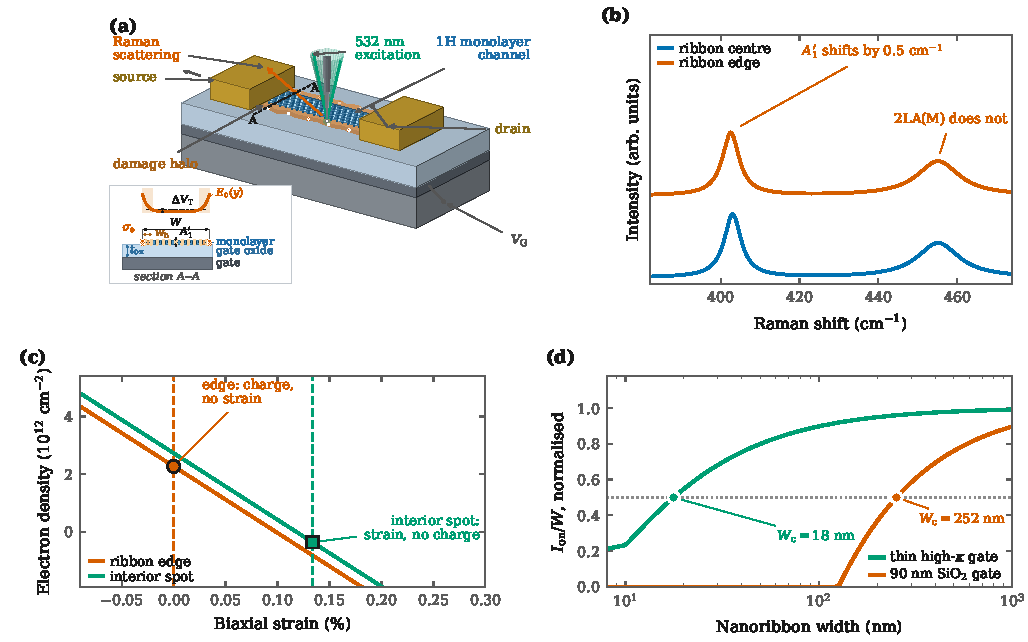
\includegraphics[width=\textwidth]{../figs/fig_abstract.pdf}
\caption{Fixed edge charge in a monolayer nanoribbon transistor, read out
from two Raman phonons. (a) The device: a monolayer ribbon of width $W$
between metal contacts on a gated stack, with the strip of process damage left
by patterning and the fixed charge $\sigma_{\rm e}$ that accumulates at the
etched edges; a tip-enhanced Raman probe samples the ribbon with about ten
nanometre resolution. (b) At the edge the $A_1'$ mode redshifts while the
2LA(M) overtone does not. (c) Each mode gives one constraint in the
strain-charge plane; they intersect at finite carrier density and zero strain
for the edge, and at finite strain and zero charge for an interior
inhomogeneity. (d) The edge charge produces a width-dependent threshold shift,
so the width at which the on-current per unit width halves depends strongly on
the gate stack. Curves are normalised to the value at 4~$\mu$m, the
wide-channel reference used to define $W_{\rm c}$, which lies beyond the
plotted range.}
\label{fig:overview}
\end{figure*}

Two-dimensional semiconductors are the leading channel candidates for
nanosheet and gate-all-around transistors beyond
silicon,\cite{Pal2024,Yin2024,Tang2025,Kim2025} and monolayer nanoribbon
devices have now been demonstrated at channel widths down to 25~nm, and at
current densities above 500~$\mu$A/$\mu$m in wider ribbons.\cite{Pena2026} As the width
shrinks, an increasing fraction of the channel lies within a few nanometres of
an etched edge, and the question of what physically stops the scaling becomes
pressing. Several candidates have been proposed: geometric edge roughness,
conducting edge states,\cite{Wu2016} process-induced damage extending well
beyond the patterned line,\cite{LiuHIM2025} and fixed charge trapped at the
edge, which was invoked long ago to explain a depletion-to-enhancement
transition observed when nanoribbons were trimmed below about
200~nm.\cite{LiuEDL2012} Recent tip-enhanced Raman imaging found a small
redshift of the out-of-plane $A_1'$ phonon at MoS$_2$ nanoribbon edges and
suggested that it was consistent with fixed negative charge, but did not
quantify it.\cite{Krayev2026} No measured value of the edge charge density in
a dichalcogenide nanoribbon exists, and without one the width limit cannot be
predicted. Figure~\ref{fig:overview} shows the device and summarises the
argument developed here.

The difficulty is that a phonon frequency responds to strain and to carrier
density at once. Etched edges are expected to carry both: elastic relaxation
of the free boundary, and charge transfer from dangling bonds and adsorbates.
A single mode therefore cannot separate them. The strain-doping correlation
plot solves this problem for graphene using two modes with different
Gr\"uneisen parameters,\cite{Lee2012graphene} and the same idea has been
applied to monolayer MoS$_2$ with the $E'$ and $A_1'$
pair.\cite{Michail2016} That pair is poorly conditioned for the present
purpose, because both are zone-centre optical phonons with similar and small
Gr\"uneisen parameters. Here we use a different pair, the first-order $A_1'$
mode and the disorder-activated 2LA(M) acoustic overtone, whose strain lever
arms differ by a factor of about four. The optical lever arm has been measured
directly under biaxial strain; the acoustic one has not, and we compute it
from first principles.

\emph{First-principles phonon response.} Deformation constants are computed
with periodic density functional theory in PySCF,\cite{Sun2020} using the PBE
functional,\cite{Perdew1996} Goedecker-Teter-Hutter
pseudopotentials\cite{Goedecker1996,Hartwigsen1998} and a DZVP-MOLOPT
basis,\cite{VandeVondele2007} on the four common 1H monolayers. The $A_1'$
normal coordinate is the chalcogen half-thickness itself, so its force
constant and its relaxed value follow together from the curvature and the
minimum of a three-point scan of that coordinate, repeated at three biaxial
strains; the in-plane $E'$ mode uses a symmetry-adapted frozen displacement
evaluated at both signs, so the force constant comes from a symmetric second
difference. A five-point biaxial strain sweep gives the elastic constant, its
strain derivative, and the deformation potential of the $K$-point gap.

Figure~\ref{fig:dft}(a) compares the computed mode Gr\"uneisen parameters with
the direct biaxial-strain measurements that exist, which cover both optical
modes of MoS$_2$ and the $A_1'$ mode of WSe$_2$.\cite{Michail2024} No
equivalent biaxial measurement has been published for WS$_2$ or MoSe$_2$. The calculated values lie above
the measured ones by up to a factor of two for MoS$_2$, which is the expected
sense of a substrate-bending experiment in which only part of the applied
strain reaches the monolayer; that same work quantifies the strain transfer
loss.\cite{Michail2024} Since the separation below depends on the \emph{ratio}
of two lever arms, we use the calculated values for both so that they are
internally consistent, and show that the result is unchanged if the measured
optical value is used instead. As an independent check on the deformation
response of the electronic structure,
Fig.~\ref{fig:dft}(b) plots the computed strain derivative of the $K$-point
gap against the measured A-exciton gauge factors of the same four
materials;\cite{Henriquez2023} the two track each other across the family
without any adjustment.

The acoustic branch behaves very differently from the optical modes. Because
the zone-edge longitudinal acoustic frequency scales as the square root of the
in-plane elastic constant, its Gr\"uneisen parameter follows from the strain
dependence of that constant, and we obtain $\gamma_{\rm LA}=\GammaLA$ for
MoS$_2$. The 2LA(M) overtone at $2\omega_{\rm LA}$ therefore shifts by
$\dwTwoLA$~cm$^{-1}$ per percent of biaxial strain, against
$\dwAeps$~cm$^{-1}$ per percent for $A_1'$, a lever-arm ratio of
\LeverRatio\ (Fig.~\ref{fig:dft}(c)). This is the property that makes the
pair useful: a strain large enough to move $A_1'$ measurably moves the
overtone by several times more. Carrier density acts the other way
round. Gated Raman measurements give a softening of $A_1'$ of
2.2~cm$^{-1}$ per $10^{13}$~cm$^{-2}$ of electrons, a consequence of the
symmetry-selective coupling of the out-of-plane mode to the $K$-valley
electron density.\cite{Chakraborty2012} No gated measurement of the 2LA(M)
coefficient exists, so we do not assume it vanishes but bound it: allowing the
overtone to renormalise with carrier density at up to half the frequency
scaled $A_1'$ rate changes the recovered edge charge by only
\OvertoneBound\%. The two channels are therefore close to independent.

\begin{figure*}[!tb]
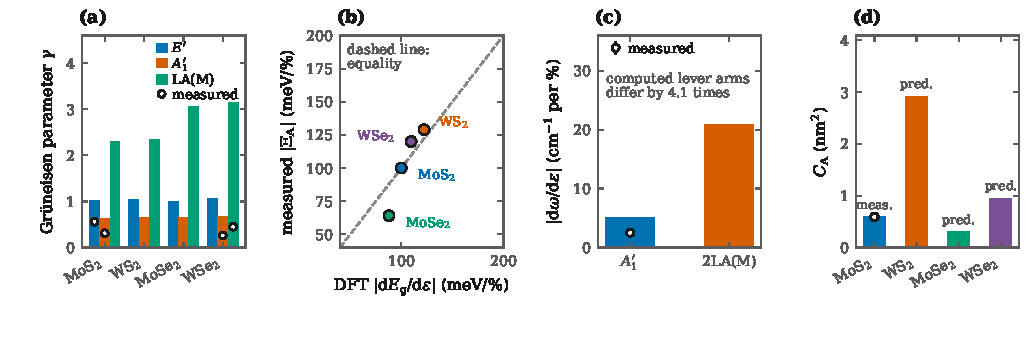
\includegraphics[width=\textwidth]{../figs/fig1.pdf}
\caption{First-principles deformation response. (a) Mode Gr\"uneisen
parameters from symmetric frozen-phonon calculations under biaxial strain,
compared with direct measurements. (b) Computed strain derivative of the
$K$-point gap against the measured A-exciton gauge factor for the same four
materials; the dashed line is equality. (c) Strain sensitivity of the two
Raman channels used here. (d) Disorder-activated Raman calibration constant:
measured for MoS$_2$, predicted here for the other three materials.}
\label{fig:dft}
\end{figure*}

\emph{Edge charge from published nanoscale spectra.} Tip-enhanced Raman maps
of lithographically patterned monolayer MoS$_2$ nanoribbons report two
distinct signatures.\cite{Krayev2026} At the ribbon edges the $A_1'$ mode
redshifts by 0.5~cm$^{-1}$ while the 2LA(M) overtone does not move. At an
interior inhomogeneity of 50 to 100~nm the overtone redshifts by
2.8~cm$^{-1}$ and $A_1'$ by 0.6~cm$^{-1}$, with a higher overtone intensity.
Solving the two-channel system with the constants above gives, at the edge,
$n=\EdgeN$~cm$^{-2}$ of electrons with a strain of
$\EdgeStrain\pm\EdgeStrainErr$\%, and at the interior spot
$\varepsilon=\SpotStrain\pm\SpotStrainErr$\%\ of tension with no significant
charge. Two very different pieces of physics, an electronic one at the
boundary and a mechanical one in the interior, are separated by the same
measurement.

The edge assignment does not depend on the calculated acoustic Gr\"uneisen
parameter. Because the overtone is measured not to shift, the strain is pinned
near zero for any value of $\gamma_{\rm LA}$, and the whole of the $A_1'$
shift must be electronic; Fig.~\ref{fig:edge}(a) shows the recovered edge
state as $\gamma_{\rm LA}$ is scanned from 0.4 to 2.6, which brackets the
plausible range for MoS$_2$. A one-mode analysis could have
assigned the same shift to \NaiveStrain\%\ of tension instead, which the
overtone excludes because such a strain would have moved 2LA(M) by
\NaiveTwoLA~cm$^{-1}$.

Two caveats attach to the sign and the environment of this number. The
coefficient used to convert the frequency shift into a density is measured for
free conduction-band electrons, so what the spectrum reports is a local excess
of band carriers; in an unbiased sample charge neutrality requires an equal
density of ionised edge states to supply them, and it is those states that
remain when the device is gated. The sign is set by the environment rather
than by the edge itself: the ribbons in question were transferred onto gold,
which donates electrons, whereas nano-optical measurements of MoS$_2$ edges on
oxide report the opposite sense, an edge that is locally
depleted.\cite{Su2019,Sousa2024} What transfers between environments is the
magnitude, of order $10^{12}$~cm$^{-2}$ within about ten nanometres of the
boundary, and it is the magnitude that governs the electrostatics below.

Converting to a line density uses the width over which the excess is
distributed. Tip-enhanced Raman resolves about 10~nm, and nano-optical work
places the electronic edge region between 5 and 20~nm on
oxide,\cite{Su2019,Wu2016} so we take $w_{\rm e}=\Wedge$~nm, giving
$\sigma_{\rm e}=\SigmaLine$~cm$^{-1}$ and a threshold shift for a ribbon of
width $W$ of
\begin{equation}
\Delta V_{\rm T}=\frac{2q\sigma_{\rm e}}{C_{\rm ox}W}.
\label{eq:dvt}
\end{equation}

Equation~(\ref{eq:dvt}) contains no adjustable parameter beyond
$\sigma_{\rm e}$ and the oxide capacitance, so it can be checked against an
experiment performed more than a decade before the spectroscopy. Figure~\ref{fig:edge}(b) shows the predicted
shift for four gate stacks. On a 300~nm back-gate oxide it reaches
\dVTLiu~V at $W=200$~nm, comparable to the several-volt threshold movement
observed when MoS$_2$ nanoribbons are trimmed through that
width.\cite{LiuEDL2012} On a
high-$\kappa$ stack with an equivalent oxide thickness of 1.5~nm the same
charge produces only \dVTHfO~V at $W=25$~nm, which is why modern nanoribbon
devices show no width-driven threshold shift.\cite{Pena2026} Fixed edge charge
is not an intrinsic barrier to scaling; it is a barrier only when the gate is
weakly coupled.

Carrying the recovered edge charge into a transport model connects it to the
measured devices. We combine the phonon-limited mobility with neutral
point-defect and screened interface-charge scattering, close the model with the
measured monolayer MoS$_2$ saturation velocity,\cite{Smithe2018} and apply
Eq.~(\ref{eq:dvt}) to the gate overdrive, taking $V_{\rm ov}=\Vov$~V,
$V_{\rm DS}=1$~V and a 300~nm channel to match the measured devices. This
gives \IonMoSTwentyfive\ and \IonMoSSeventyfive~$\mu$A/$\mu$m for MoS$_2$
ribbons of width 25 and 75~nm on the high-$\kappa$ stack, against 310 and
400~$\mu$A/$\mu$m measured, and \IonWSTwo~$\mu$A/$\mu$m for WS$_2$ at 43~nm
against 420~$\mu$A/$\mu$m (Fig.~\ref{fig:edge}(c)).\cite{Pena2026} The WS$_2$ value is overestimated by
about \IonWSover\%, and the p-type WSe$_2$ prediction lies well above the measurement
because those devices are limited by contact resistance rather than by the
channel.\cite{Sun2026,Mondal2024}

\begin{figure*}[!tb]
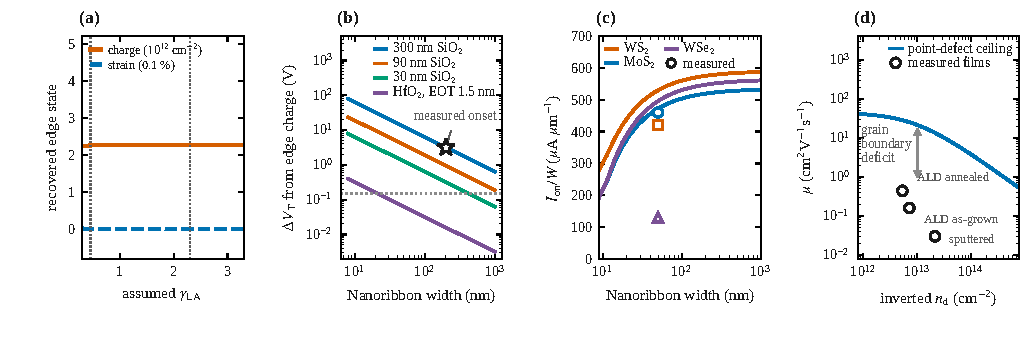
\includegraphics[width=\textwidth]{../figs/fig2.pdf}
\caption{Edge charge and its electrostatic signature. (a) Recovered edge
carrier density and strain as the assumed acoustic Gr\"uneisen parameter is
scanned; the assignment is fixed by the unshifted overtone. (b) Threshold
shift predicted by Eq.~(\ref{eq:dvt}) for four gate stacks; the dotted line is
ten per cent of the gate overdrive and the star marks the width at which a
width-driven threshold shift was first reported.\cite{LiuEDL2012} (c) Predicted and measured on-current per unit
width; measured points are the high-$\kappa$-gated devices of
Ref.~\onlinecite{Pena2026}. (d) Defect densities inverted from the disorder-activated Raman ratio
of published films, against their measured mobility and the point-defect
ceiling.}
\label{fig:edge}
\end{figure*}

\begin{figure*}[!tb]
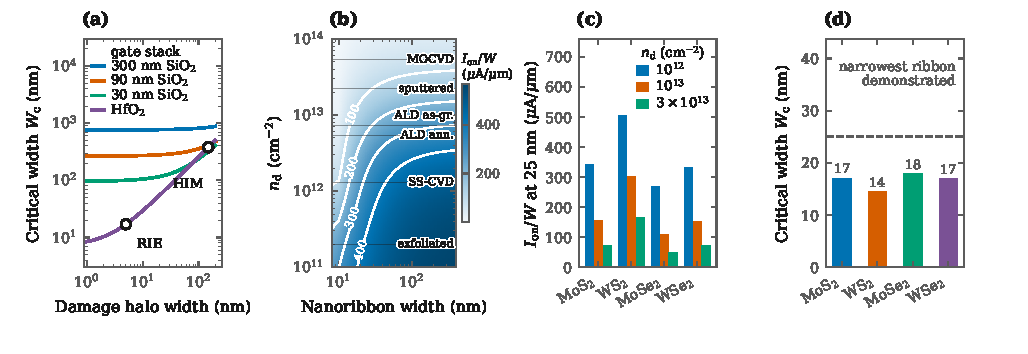
\includegraphics[width=\textwidth]{../figs/fig3.pdf}
\caption{What sets the width limit. (a) Critical width against
process-induced damage halo for four gate stacks; symbols mark reported halo
widths for reactive-ion etching (RIE) and helium-ion milling (HIM). (b) On-current per
unit width over ribbon width and defect density; horizontal lines mark
representative growth technologies, the two atomic-layer-deposited and the two
sputtered values inverted here from published Raman ratios and the remaining
two taken from the literature. (c) Screening of the four
materials at a 25~nm width for three defect densities. (d) Critical width of
the four materials; the dashed line is the narrowest ribbon demonstrated to
date.}
\label{fig:limit}
\end{figure*}

\emph{What sets the width limit.} The second control on scaling is the damage
halo left by patterning, a strip beside each edge with an elevated defect
density. Reported halo widths span two orders of magnitude, from a few
nanometres for optimised reactive-ion etching\cite{Pena2026} to about 150~nm
for helium-ion milling.\cite{LiuHIM2025} Defining the critical width
$W_{\rm c}$ as the width at which the on-current per unit width falls to half
of its wide-channel value at $V_{\rm ov}=\Vov$~V,
Fig.~\ref{fig:limit}(a) plots $W_{\rm c}$ against halo width for the four gate
stacks. The two causes act in different regimes and are worth separating. On a
thin high-$\kappa$ gate with a narrow halo the halo dominates, contributing
\WcHaloHfO~nm against \WcChgHfO~nm from the edge charge, and
$W_{\rm c}=\WcRIE$~nm; the demonstrated 25~nm ribbons sit just above it. For a
wide halo the critical width tracks the halo directly and reaches
\WcHIM~nm. On a thick oxide the edge-charge term takes over and $W_{\rm c}$
saturates near \WcChgSiOThirty~nm for a 30~nm oxide, no matter how clean the
etch is. The distinction matters in practice, because a width-dependent
threshold offset can be partly compensated by design, whereas the transport
degradation of the damaged halo cannot. The edge-charge branch scales with the
assumed edge width, moving $W_{\rm c}$ on the high-$\kappa$ stack from
\WcHfOwFive\ to \WcHfOwTwenty~nm as $w_{\rm e}$ is varied from 5 to 20~nm,
whereas the halo branch is unaffected.

As-grown film quality enters differently. To make that explicit we invert the
disorder-activated Raman ratio of published atomic-layer-deposited and
sputtered MoS$_2$ films,\cite{Nattoo2025} using the relation
$I_{\rm LA}/I_{A_1'}=C_{\rm A}n_{\rm d}$ calibrated on ion-irradiated
monolayers.\cite{Mignuzzi2015} Those films span $n_{\rm d}$ from $\ndALDan$ to
$\ndSPag$~cm$^{-2}$, and their measured mobilities lie between \DeficitLo\ and
\DeficitHi\ times below the point-defect ceiling (Fig.~\ref{fig:edge}(d)), the
expected signature of nanocrystalline material in which grain boundaries rather
than point defects dominate transport.\cite{vanderZande2013} Over that same
range of defect density the on-current at a fixed 25~nm width falls by a factor
of \IdropFilm\ (Fig.~\ref{fig:limit}(b) and (c)), while $W_{\rm c}$ moves by
only \WcDriftFilm\%. Film quality therefore sets how much current a
ribbon delivers, whereas the patterning process and the gate stack set how
narrow it can usefully be made.

Because the calibration constant $C_{\rm A}$ has been measured only for
MoS$_2$, we also predict it for the rest of the family. In the double
resonance picture the disorder-activated intensity relative to the first-order
line scales as $|D|^2/(\omega_{\rm LA}^2\Delta^2)$, with $D$ the gap
deformation potential computed above, $\omega_{\rm LA}$ the zone-edge acoustic
frequency and $\Delta$ the detuning of the laser from the A exciton. Anchoring
on the MoS$_2$ value $0.59\pm0.03$~nm$^2$ at 532~nm,\cite{Mignuzzi2015} this
gives $C_{\rm A}=\CAWSTwo$, \CAMoSeTwo\ and \CAWSeTwo~nm$^2$ for WS$_2$,
MoSe$_2$ and WSe$_2$ (Fig.~\ref{fig:dft}(d)), testable predictions that would
let the same ion-irradiation calibration be skipped for those materials.
Screening the family at a 25~nm width puts WS$_2$ first on current density and
also gives it the smallest critical width, so it is the most scalable of the
four on both counts (Fig.~\ref{fig:limit}(c) and (d)); the ordering follows the
effective masses and phonon-limited mobilities.\cite{Jin2014,Ha2024}

Both separations above are two-observable weighted least squares with a broad
prior. The same forward model extends to a full hyperspectral image, where
defect density, strain and carrier density are recovered jointly; that
extension uses a physics-guided adjoint solver and is verified on synthetic
data in the supplementary material, together with the complete parameter
provenance. The code is openly available.

Several limitations bound these conclusions. The electronic structure is
computed at the PBE level without spin-orbit coupling, so we use published
spin-orbit-resolved effective masses\cite{Jin2014,Kormanyos2015} and take only
strain derivatives from our own calculations. The edge charge is inferred from
a single published data set on one material, on ribbons supported by gold, and
assumes the excess is uniform over an edge width of \Wedge~nm; the sign is
environment dependent and the reported density scales inversely with the
measured $A_1'$ doping coefficient. A capacitance measurement on a width
series would test all three.
The predicted calibration constants for WS$_2$, MoSe$_2$ and WSe$_2$ rest on a
double-resonance scaling argument and await measurement. The transport layer
contains two constants fixed once against published results, the neutral
defect potential and the interface charge density of each gate stack, and it
does not include contact resistance, so the predicted currents are
channel-limited ceilings.

In summary, the quantity that limits width scaling in monolayer dichalcogenide
nanoribbon transistors is fixed charge at the etched edge, and it can be read
out non-destructively from the ratio of two phonon responses. First-principles
Gr\"uneisen parameters make the $A_1'$ and 2LA(M) pair an orthogonal probe of
charge and strain, and applying it to published tip-enhanced Raman data yields
a local excess of $\EdgeN$~cm$^{-2}$ of band electrons at MoS$_2$ nanoribbon
edges, and therefore an equal density of fixed ionised edge states, together
with a clean separation of a purely mechanical interior inhomogeneity. Charge of that size
accounts for a decade-old depletion-to-enhancement observation and, together
with the patterning damage halo, sets a critical width ranging from
\WcRIE~nm on a thin high-$\kappa$ gate to several hundred nanometres for a
weak gate or a damaging etch, while depending only weakly on as-grown defect
density. The practical consequence is
that width scaling is bought with gate coupling and gentle patterning rather
than with better films, and that both can be checked optically before a device
is built.


\section*{Author declarations}
\noindent\textbf{Conflict of interest.} The authors have no conflicts to
disclose.

\noindent\textbf{Use of AI tools.} The authors used AI-assisted writing tools,
including Chat GPT and Gemini, solely to improve the clarity, readability, and
language of the manuscript. All scientific ideas, technical content,
theoretical analyses, experimental design, and conclusions were conceived,
developed, and verified independently by the authors without AI assistance.

\noindent\textbf{Author contributions.} \textbf{Tanvir M. Mahim:}
Conceptualization (lead); Methodology (lead); Software (lead); Formal analysis
(lead); Writing -- original draft (lead). \textbf{M. Mosaddequr Rahman:}
Supervision (lead); Validation (equal); Writing -- review and editing (equal).

\section*{Data availability}
The data that support the findings of this study are openly available in Zenodo
at \url{https://doi.org/10.5281/zenodo.21670316}, reference
number~\onlinecite{Mahim2026data}. That deposit contains the raw
first-principles output, every digitised published measurement used here as a
flat file with its source stated, the machine-readable results file from which
every number, table and figure in this article is generated, and the figures as
published. The complete code base, including the density functional theory
drivers, the forward model, the adjoint solver, the transport layer and the
scripts that regenerate every figure and every number in this article, is
openly available at
\url{https://github.com/Tanvir-Mahmud-Mahim/Width-scaling-in-monolayer-semiconductor-nanoribbon-transistors}
and is archived in the same Zenodo deposit.

\nocite{aip41Control}
\bibliographystyle{aipnum4-1}
\bibliography{refs}

\end{document}
